%% NXP eIQ Model Zoo — LaTeX Beamer Presentation
%% Compile: pdflatex NXP_ModelZoo_Slides.tex
\documentclass[aspectratio=169]{beamer}

%% ── Packages ─────────────────────────────────────────────────────────────────
\usepackage[utf8]{inputenc}
\usepackage[T1]{fontenc}
\usepackage{lmodern}
\usepackage{amsmath,amssymb}
\usepackage{graphicx}
\usepackage{booktabs}
\usepackage{colortbl}
\usepackage{xcolor}
\usepackage{tikz}
\usepackage{pgfplots}
\usepackage{listings}
\usepackage{array}
\usepackage{multirow}
\usepackage{hyperref}
\pgfplotsset{compat=1.18}
\usetikzlibrary{arrows.meta,shapes,positioning,fit,backgrounds,calc,decorations.pathreplacing}

%% ── NXP Brand Colors ─────────────────────────────────────────────────────────
\definecolor{NXPOrange}{RGB}{255,102,0}
\definecolor{NXPBlue}{RGB}{0,56,101}
\definecolor{NXPDark}{RGB}{30,30,50}
\definecolor{NXPGray}{RGB}{120,120,120}
\definecolor{NXPLightBlue}{RGB}{0,120,200}
\definecolor{NXPLightGray}{RGB}{230,230,230}

%% ── Theme Setup ──────────────────────────────────────────────────────────────
\usetheme{Madrid}
\usecolortheme{default}

\setbeamercolor{palette primary}{bg=NXPBlue,fg=white}
\setbeamercolor{palette secondary}{bg=NXPDark,fg=white}
\setbeamercolor{palette tertiary}{bg=NXPOrange,fg=white}
\setbeamercolor{palette quaternary}{bg=NXPBlue!80,fg=white}
\setbeamercolor{structure}{fg=NXPBlue}
\setbeamercolor{frametitle}{bg=NXPBlue,fg=white}
\setbeamercolor{title}{bg=NXPBlue,fg=white}
\setbeamercolor{block title}{bg=NXPOrange,fg=white}
\setbeamercolor{block body}{bg=NXPLightGray,fg=NXPDark}
\setbeamercolor{alerted text}{fg=NXPOrange}
\setbeamercolor{itemize item}{fg=NXPOrange}
\setbeamercolor{itemize subitem}{fg=NXPBlue}
\setbeamercolor{enumerate item}{fg=NXPOrange}

%% ── Code listing style ───────────────────────────────────────────────────────
\lstset{
  basicstyle=\ttfamily\tiny,
  keywordstyle=\color{NXPOrange}\bfseries,
  commentstyle=\color{NXPGray},
  stringstyle=\color{NXPBlue},
  backgroundcolor=\color{NXPDark!8},
  frame=single,framerule=0.4pt,
  breaklines=true,
  numbers=none,
  xleftmargin=4pt,xrightmargin=4pt,
}

%% ── TikZ node styles ─────────────────────────────────────────────────────────
\tikzset{
  pbox/.style={draw=NXPBlue,fill=NXPBlue!12,rounded corners=4pt,minimum height=8mm,text width=2.1cm,align=center,font=\scriptsize},
  obox/.style={draw=NXPOrange,fill=NXPOrange!12,rounded corners=4pt,minimum height=8mm,text width=2.1cm,align=center,font=\scriptsize},
  gbox/.style={draw=NXPGray,fill=NXPGray!10,rounded corners=4pt,minimum height=8mm,text width=2.1cm,align=center,font=\scriptsize},
  dbox/.style={draw=NXPDark,fill=NXPDark!8,rounded corners=4pt,minimum height=8mm,text width=2.5cm,align=center,font=\scriptsize},
  arr/.style={-{Stealth[length=4pt]},NXPBlue,thick},
  oarr/.style={-{Stealth[length=4pt]},NXPOrange,thick},
}

%% ── Title & metadata ─────────────────────────────────────────────────────────
\title[NXP eIQ Model Zoo]{\textbf{NXP eIQ\textsuperscript{\textregistered} Model Zoo}\\TFLite-First Embedded AI for i.MX \& MCX Platforms}
\subtitle{Pre-trained TensorFlow Lite INT8 Models for MPU, MCU, and NPU Deployment}
\author{NXP Semiconductors}
\institute{\texttt{github.com/NXP/eiq-model-zoo}}
\date{2026}

%% ═════════════════════════════════════════════════════════════════════════════
\begin{document}

%% ── Title ────────────────────────────────────────────────────────────────────
\begin{frame}
  \titlepage
\end{frame}

%% ── Contents ─────────────────────────────────────────────────────────────────
\begin{frame}{Outline}
  \tableofcontents[hideallsubsections]
\end{frame}

%% ═══════════════════════════════════════════════════════════════════
\section{Overview}
%% ═══════════════════════════════════════════════════════════════════

\begin{frame}{NXP eIQ\textsuperscript{\textregistered} Model Zoo — At a Glance}
  \begin{columns}[T]
    \column{0.5\textwidth}
      \begin{block}{What is it?}
        A curated collection of \alert{pre-trained ML models} for embedded deployment on NXP products, delivered as \textbf{conversion recipes} that produce TFLite INT8 models.
      \end{block}
      \vspace{4pt}
      \begin{block}{Key Numbers}
        \begin{itemize}
          \item \alert{$\sim$35 models} across 3 domains
          \item \alert{9 vision tasks} (most of any zoo studied)
          \item \alert{5 hardware platforms}: MPU + MCU
          \item \alert{1 format}: TensorFlow Lite INT8
          \item Docker-based reproducible recipes
        \end{itemize}
      \end{block}
    \column{0.48\textwidth}
      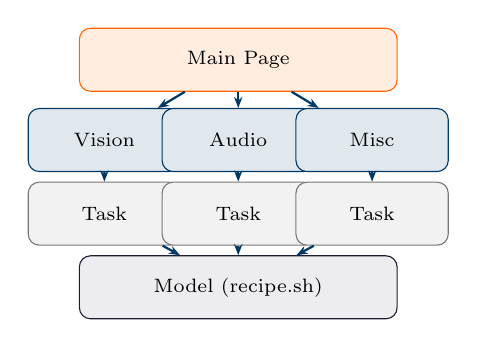
\begin{tikzpicture}[scale=0.85,font=\scriptsize]
        \node[obox,text width=3.8cm] (ml) at (0,2.2) {Main Page};
        \node[pbox,text width=1.7cm] (v)  at (-2,1.0) {Vision};
        \node[pbox,text width=1.7cm] (a)  at (0,1.0)  {Audio};
        \node[pbox,text width=1.7cm] (m)  at (2,1.0)  {Misc};
        \node[gbox,text width=1.7cm] (t1) at (-2,-0.1){Task};
        \node[gbox,text width=1.7cm] (t2) at (0,-0.1) {Task};
        \node[gbox,text width=1.7cm] (t3) at (2,-0.1) {Task};
        \node[dbox,text width=3.8cm] (mo) at (0,-1.2) {Model (recipe.sh)};
        \draw[arr] (ml)--(v); \draw[arr] (ml)--(a); \draw[arr] (ml)--(m);
        \draw[arr] (v)--(t1); \draw[arr] (a)--(t2); \draw[arr] (m)--(t3);
        \draw[arr] (t1)--(mo); \draw[arr] (t2)--(mo); \draw[arr] (t3)--(mo);
      \end{tikzpicture}
  \end{columns}
\end{frame}

\begin{frame}{What Makes NXP eIQ Model Zoo Unique}
  \begin{columns}[T]
    \column{0.48\textwidth}
      \begin{block}{vs.\ TI EdgeAI Model Zoo}
        \begin{itemize}\small
          \item TI: 180+ models, vision only, ONNX+TFLite+TVM
          \item NXP: $\sim$35 models, multi-domain, \textbf{TFLite only}
          \item NXP has: super resolution, low-light enhancement, instance segmentation, EEG/BCI, full speech recognition
          \item NXP targets MPU class (Linux) \emph{and} MCU class
        \end{itemize}
      \end{block}
      \vspace{4pt}
      \begin{block}{vs.\ ADI Model Zoo}
        \begin{itemize}\small
          \item ADI: 15 models, AI8X proprietary format
          \item NXP: 35 models, industry-standard TFLite
          \item ADI: ultra-low power MCU ($<$1mW)
          \item NXP: NPU-accelerated MPU (2.3 TOPS)
        \end{itemize}
      \end{block}
    \column{0.48\textwidth}
      \begin{block}{Unique Differentiators}
        \begin{enumerate}\small
          \item \alert{Recipe system} — Docker-based, reproducible FP32$\to$INT8
          \item \alert{Ethos-U65 NPU} support on i.MX 93 via Vela compiler
          \item \alert{EEG/BCI model} — only zoo with brain-computer interface model
          \item \alert{Super resolution \& low-light enhancement} tasks
          \item \alert{Full ASR} (Wav2Letter, WER 7.2\%)
          \item \alert{Instance segmentation} (YOLACT-Edge)
        \end{enumerate}
      \end{block}
  \end{columns}
\end{frame}

%% ═══════════════════════════════════════════════════════════════════
\section{Target Hardware}
%% ═══════════════════════════════════════════════════════════════════

\begin{frame}{Supported Hardware Platforms}
  \centering
  \small
  \begin{tabular}{llll}
    \toprule
    \textbf{Device} & \textbf{Family} & \textbf{Core} & \textbf{Key Feature} \\
    \midrule
    \rowcolor{NXPBlue!10}
    i.MX 8M Plus & MPU & Cortex-A53 $\times$4 + NPU & \alert{2.3 TOPS NPU}, DDR4, Linux \\
    i.MX 93      & MPU & Cortex-A55 $\times$2 + Ethos-U65 & \alert{1 TOPS NPU}, ultra-low power \\
    \rowcolor{NXPBlue!10}
    i.MX RT1170  & MCU & Cortex-M7 + M4 & 1\,GHz, 2\,MB SRAM \\
    i.MX RT1050/1060 & MCU & Cortex-M7 & 600\,MHz, constrained \\
    \rowcolor{NXPBlue!10}
    MCX N947     & MCU & Cortex-M33 + NPU & BLE 5.3, low power \\
    \bottomrule
  \end{tabular}
  \vspace{8pt}
  \begin{block}{Key deployment note}
    i.MX 93 requires \textbf{Vela compiler} for Ethos-U65 NPU acceleration.
    BSP $\geq$ LF6.1.36\_2.1.0 supports online Vela compilation via the Ethos-U Delegate.
  \end{block}
\end{frame}

\begin{frame}{Platform Performance Comparison}
  \centering
  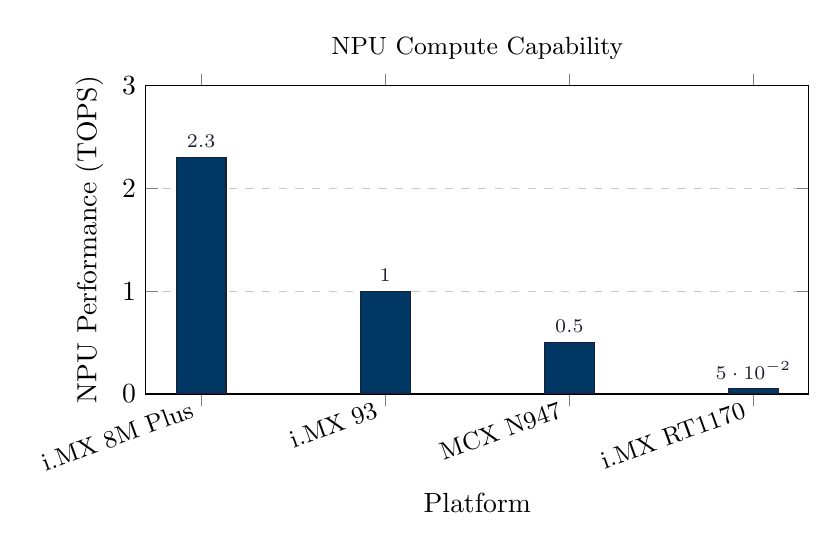
\begin{tikzpicture}
    \begin{axis}[
      width=10cm, height=5.5cm,
      ybar, bar width=18pt,
      xlabel={Platform},
      ylabel={NPU Performance (TOPS)},
      symbolic x coords={i.MX 8M Plus, i.MX 93, MCX N947, i.MX RT1170},
      xtick=data,
      x tick label style={rotate=20,anchor=east,font=\small},
      ymin=0, ymax=3.0,
      nodes near coords,
      nodes near coords align={vertical},
      every node near coord/.style={font=\scriptsize,color=NXPDark},
      bar shift=0pt,
      ymajorgrids=true,
      grid style={dashed,NXPGray!40},
      title={\small NPU Compute Capability},
    ]
    \addplot[fill=NXPBlue,draw=NXPDark] coordinates {
      (i.MX 8M Plus,2.3)
      (i.MX 93,1.0)
      (MCX N947,0.5)
      (i.MX RT1170,0.05)
    };
    \end{axis}
  \end{tikzpicture}
  \vspace{2pt}
  \begin{itemize}\small
    \item i.MX RT1170: CPU-only TFLite inference (no dedicated NPU)
    \item MCX N947: integrated ML accelerator, lower power envelope
    \item i.MX 8M Plus: full Linux, \alert{highest throughput for MPU tasks}
  \end{itemize}
\end{frame}

\begin{frame}{eIQ Toolkit Deployment Architecture}
  \centering
  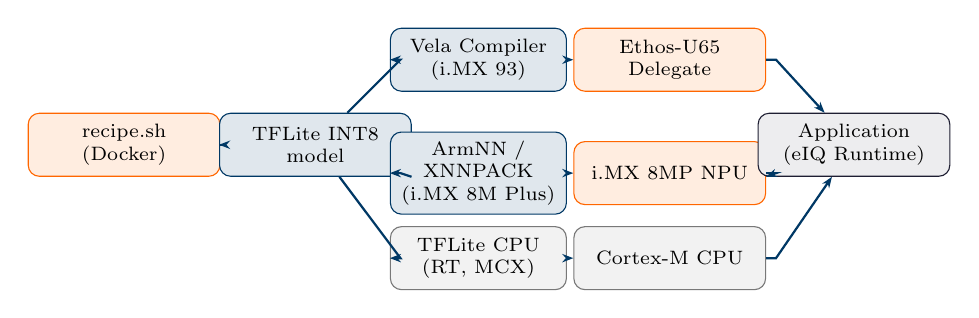
\begin{tikzpicture}[scale=0.9,font=\scriptsize]
    %% Source
    \node[obox,text width=2.2cm] (recipe) at (-5.5,0) {recipe.sh\\(Docker)};
    \node[pbox,text width=2.2cm] (tflite) at (-2.8,0) {TFLite INT8\\model};
    %% Branch
    \node[pbox,text width=2.0cm] (vela)  at (-0.5, 1.2) {Vela Compiler\\(i.MX 93)};
    \node[pbox,text width=2.0cm] (eiq8m) at (-0.5,-0.4) {ArmNN / XNNPACK\\(i.MX 8M Plus)};
    \node[gbox,text width=2.0cm] (cpu)   at (-0.5,-1.6) {TFLite CPU\\(RT, MCX)};
    %% Runtime
    \node[obox,text width=2.2cm] (rt)    at (2.2, 1.2) {Ethos-U65\\Delegate};
    \node[obox,text width=2.2cm] (npu8m) at (2.2,-0.4) {i.MX 8MP NPU};
    \node[gbox,text width=2.2cm] (cpurt) at (2.2,-1.6) {Cortex-M CPU};
    %% App
    \node[dbox,text width=2.2cm] (app)   at (4.8, 0) {Application\\(eIQ Runtime)};
    %% Arrows
    \draw[arr] (recipe)--(tflite);
    \draw[arr] (tflite)--(-1.6,1.2)--(vela);
    \draw[arr] (tflite)--(-1.6,-0.4)--(eiq8m);
    \draw[arr] (tflite)--(-1.6,-1.6)--(cpu);
    \draw[arr] (vela)--(rt);
    \draw[arr] (eiq8m)--(npu8m);
    \draw[arr] (cpu)--(cpurt);
    \draw[arr] (rt)--(3.7,1.2)--(app);
    \draw[arr] (npu8m)--(3.7,-0.4)--(app);
    \draw[arr] (cpurt)--(3.7,-1.6)--(app);
  \end{tikzpicture}
\end{frame}

%% ═══════════════════════════════════════════════════════════════════
\section{Model Domains}
%% ═══════════════════════════════════════════════════════════════════

\begin{frame}{Three Domains, Thirteen Tasks}
  \begin{columns}[T]
    \column{0.38\textwidth}
      \begin{block}{\textcolor{NXPOrange}{\textbf{Vision}} (9 tasks)}
        \begin{itemize}\scriptsize
          \item Image Classification
          \item Object Detection
          \item Semantic Segmentation
          \item Instance Segmentation
          \item Face Recognition
          \item Pose Estimation
          \item Super Resolution
          \item Low-light Enhancement
          \item Monocular Depth Estimation
        \end{itemize}
      \end{block}
    \column{0.28\textwidth}
      \begin{block}{\textcolor{NXPBlue}{\textbf{Audio}} (3 tasks)}
        \begin{itemize}\scriptsize
          \item Command Recognition (KWS)
          \item Anomaly Detection
          \item Speech Recognition (ASR)
        \end{itemize}
      \end{block}
      \vspace{6pt}
      \begin{block}{\textcolor{NXPDark}{\textbf{Misc}} (1 task)}
        \begin{itemize}\scriptsize
          \item EEG / BCI\\Motor Imagery
        \end{itemize}
      \end{block}
    \column{0.30\textwidth}
      \begin{alertblock}{Unique Tasks}
        \scriptsize
        Tasks not found in TI or ADI zoos:
        \begin{itemize}
          \item Super Resolution
          \item Low-light Enhancement
          \item Instance Segmentation
          \item Full ASR (Wav2Letter)
          \item \textbf{EEG/BCI Classification}
          \item Monocular Depth
        \end{itemize}
      \end{alertblock}
  \end{columns}
\end{frame}

%% ═══════════════════════════════════════════════════════════════════
\section{Recipe System}
%% ═══════════════════════════════════════════════════════════════════

\begin{frame}[fragile]{The Recipe System — Reproducible TFLite Conversion}
  \begin{columns}[T]
    \column{0.52\textwidth}
      \begin{block}{What is a Recipe?}
        Each model directory contains \texttt{recipe.sh} — a shell script that:
        \begin{enumerate}\scriptsize
          \item Downloads original model (PyTorch / TF / ONNX)
          \item Converts to TFLite float
          \item Quantizes to \alert{INT8} using representative dataset
          \item Outputs ready-to-deploy \texttt{.tflite} file
        \end{enumerate}
      \end{block}
      \vspace{6pt}
      \begin{block}{Running a Recipe}
        \begin{lstlisting}[language=bash]
# Build the Docker image once
docker build -t nxp-model-zoo .

# Run any model recipe
cd tasks/vision/object-detection/yolov8
docker run --rm \
  -v "$PWD:/workspace" \
  nxp-model-zoo \
  /workspace/recipe.sh
        \end{lstlisting}
      \end{block}
    \column{0.44\textwidth}
      \begin{block}{Why Docker?}
        \begin{itemize}\scriptsize
          \item Reproducible environment (Ubuntu 20.04 + Python 3.8)
          \item Handles complex dependency chains (PyTorch $\to$ ONNX $\to$ TF $\to$ TFLite)
          \item No host environment pollution
          \item CI-friendly
        \end{itemize}
      \end{block}
      \vspace{4pt}
      \begin{alertblock}{Output}
        \scriptsize
        One \texttt{.tflite} file per recipe:
        \begin{itemize}
          \item Fully INT8 quantized
          \item INT8 input + INT8 output (most models)
          \item Some models: float32 I/O with INT8 weights
        \end{itemize}
      \end{alertblock}
  \end{columns}
\end{frame}

\begin{frame}{Quantization Pipeline \& Vela Compilation}
  \centering
  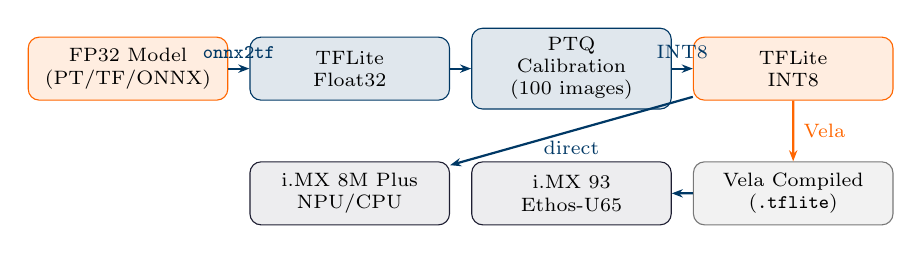
\begin{tikzpicture}[scale=0.88,font=\scriptsize]
    \node[obox,text width=2.3cm] (fp32)  at (0,0)   {FP32 Model\\(PT/TF/ONNX)};
    \node[pbox,text width=2.3cm] (tflf)  at (3.2,0) {TFLite\\Float32};
    \node[pbox,text width=2.3cm] (ptq)   at (6.4,0) {PTQ\\Calibration\\(100 images)};
    \node[obox,text width=2.3cm] (int8)  at (9.6,0) {TFLite\\INT8};
    \node[gbox,text width=2.3cm] (vela)  at (9.6,-1.8) {Vela Compiled\\(\texttt{.tflite})};
    \node[dbox,text width=2.3cm] (board) at (6.4,-1.8) {i.MX 93\\Ethos-U65};
    \node[dbox,text width=2.3cm] (imx8m) at (3.2,-1.8) {i.MX 8M Plus\\NPU/CPU};
    \draw[arr] (fp32)--(tflf) node[midway,above]{\texttt{onnx2tf}};
    \draw[arr] (tflf)--(ptq);
    \draw[arr] (ptq)--(int8) node[midway,above]{INT8};
    \draw[oarr] (int8)--(vela) node[midway,right]{Vela};
    \draw[arr] (vela)--(board);
    \draw[arr] (int8)--(imx8m) node[midway,below]{direct};
  \end{tikzpicture}
  \vspace{8pt}
  \begin{columns}[T]
    \column{0.48\textwidth}
      \small\textbf{Calibration datasets used:}
      \begin{itemize}\scriptsize
        \item COCO 2017 validation (detection/segmentation)
        \item ImageNet samples (classification)
        \item Speech Commands (audio)
      \end{itemize}
    \column{0.48\textwidth}
      \small\textbf{Vela — required for i.MX 93:}
      \begin{itemize}\scriptsize
        \item BSP $\geq$ LF6.1.36: online Vela via Ethos-U Delegate
        \item Older BSP: offline \texttt{vela model.tflite}
        \item Source: \texttt{github.com/nxp-imx/ethos-u-vela}
      \end{itemize}
  \end{columns}
\end{frame}

%% ═══════════════════════════════════════════════════════════════════
\section{Vision Models}
%% ═══════════════════════════════════════════════════════════════════

\begin{frame}{Vision — Image Classification}
  \centering\small
  \begin{tabular}{lllll}
    \toprule
    \textbf{Model} & \textbf{Dataset} & \textbf{Input} & \textbf{Top-1} & \textbf{Platforms} \\
    \midrule
    MobileNetV1      & ImageNet   & 224$\times$224 & \alert{70.9\%} & 8MP, 93, RT1x \\
    MobileNetV2      & ImageNet   & 224$\times$224 & \alert{71.8\%} & 8MP, 93, MCX \\
    MnasNet          & ImageNet   & 224$\times$224 & ---            & 8MP, 93 \\
    EfficientNet-Lite& ImageNet   & 224$\times$224 & ---            & 8MP, 93 \\
    ResNet50         & ImageNet   & 224$\times$224 & \alert{$\sim$76\%} & 8MP, 93 \\
    InceptionV4      & ImageNet   & ---            & ---            & 8MP, 93 \\
    Tiny-ResNet      & CIFAR-10   & 32$\times$32   & ---            & MCX N947 \\
    Visual Wake Word & VW COCO14  & ---            & ---            & MCX, i.MX \\
    Deepface-emotion & FER2013    & ---            & 8 classes      & 8MP, 93 \\
    \bottomrule
  \end{tabular}
  \vspace{4pt}
  \begin{itemize}\small
    \item All models: TFLite INT8, fully quantized
    \item MobileNetV2: \alert{608 MOPS}, 3.5M parameters, Keras origin
  \end{itemize}
\end{frame}

\begin{frame}{Vision — Classification: Accuracy vs.\ Complexity}
  \centering
  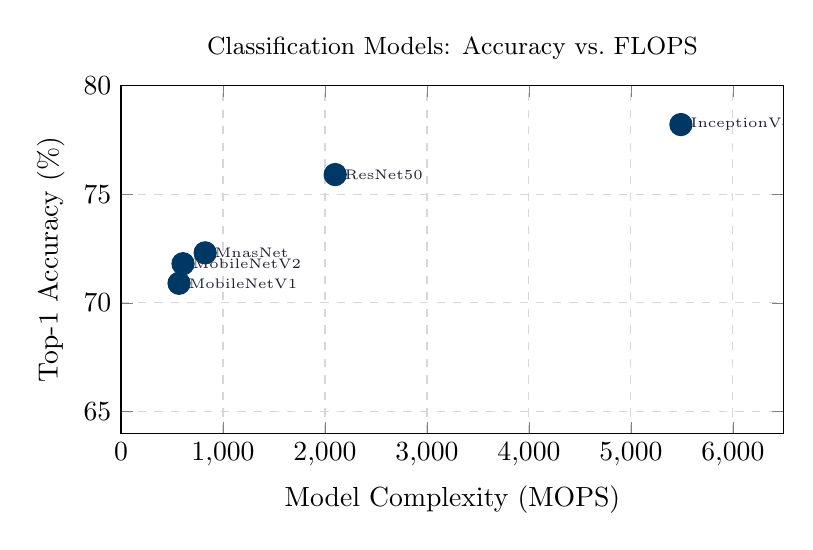
\begin{tikzpicture}
    \begin{axis}[
      width=10cm, height=6cm,
      xlabel={Model Complexity (MOPS)},
      ylabel={Top-1 Accuracy (\%)},
      xmin=0, xmax=6500,
      ymin=64, ymax=80,
      ymajorgrids, xmajorgrids,
      grid style={dashed,NXPGray!30},
      title={\small Classification Models: Accuracy vs.\ FLOPS},
    ]
    %% (MOPS, Top-1, label)
    \addplot[only marks, mark=*, mark size=4pt, NXPBlue] coordinates {
      (608, 71.8)
      (569, 70.9)
      (2100, 75.9)
      (5490, 78.2)
      (825, 72.3)
    };
    \node[font=\tiny,NXPDark,right] at (axis cs:608,71.8) {MobileNetV2};
    \node[font=\tiny,NXPDark,right] at (axis cs:569,70.9) {MobileNetV1};
    \node[font=\tiny,NXPDark,right] at (axis cs:2100,75.9) {ResNet50};
    \node[font=\tiny,NXPDark,right] at (axis cs:5490,78.2) {InceptionV4};
    \node[font=\tiny,NXPDark,right] at (axis cs:825,72.3) {MnasNet};
    \end{axis}
  \end{tikzpicture}
\end{frame}

\begin{frame}{Vision — Object Detection (11 Models)}
  \centering\scriptsize
  \begin{tabular}{llllp{2.8cm}}
    \toprule
    \textbf{Model} & \textbf{Dataset} & \textbf{Input} & \textbf{mAP} & \textbf{Platforms} \\
    \midrule
    \rowcolor{NXPBlue!8}
    YOLOv8-m        & COCO       & 320$\times$320 & \alert{50.2\%} & i.MX 8MP, 93 \\
    YOLOv5          & COCO       & ---            & ---            & i.MX 8MP, 93 \\
    \rowcolor{NXPBlue!8}
    YOLOv4-tiny     & COCO       & ---            & ---            & i.MX 8MP, 93 \\
    SSDLite MNV2    & COCO       & ---            & ---            & i.MX 8MP, 93 \\
    \rowcolor{NXPBlue!8}
    EfficientDet-L0 & COCO       & ---            & ---            & i.MX 8MP, 93 \\
    NanoDet-M       & COCO       & ---            & ---            & 8MP, 93, RT1170, RT1050 \\
    \rowcolor{NXPBlue!8}
    CenterNet       & COCO       & ---            & ---            & i.MX 8MP, 93 \\
    FastestDet      & Pascal VOC & ---            & ---            & RT1170 \\
    \rowcolor{NXPBlue!8}
    FaceDet         & WiderFace  & ---            & ---            & \textbf{All platforms} \\
    Ultraface-Slim  & WiderFace  & ---            & ---            & 8MP, 93, RT1x \\
    \rowcolor{NXPBlue!8}
    Ultraface-Ultraslim & WiderFace & ---         & ---            & MCX N947 \\
    \bottomrule
  \end{tabular}
  \vspace{4pt}
  \textbf{YOLOv8-m}: \alert{78.9B OPS}, 25.9M params, PyTorch $\to$ TFLite via Ultralytics
\end{frame}

\begin{frame}{Model-Platform Compatibility Matrix}
  \centering\scriptsize
  \newcommand{\yes}{\textcolor{NXPBlue}{\textbf{\checkmark}}}
  \newcommand{\no}{\textcolor{NXPGray}{--}}
  \begin{tabular}{lccccc}
    \toprule
    \textbf{Model} & \textbf{8M Plus} & \textbf{i.MX 93} & \textbf{RT1170} & \textbf{RT1050} & \textbf{MCX N947} \\
    \midrule
    MobileNetV1/V2    & \yes & \yes & \no  & \no  & \no  \\
    EfficientNet-Lite & \yes & \yes & \no  & \no  & \no  \\
    Tiny-ResNet       & \yes & \yes & \no  & \no  & \yes \\
    Visual Wake Word  & \yes & \yes & \no  & \no  & \yes \\
    YOLOv8-m / v5     & \yes & \yes & \no  & \no  & \no  \\
    YOLOv4-tiny       & \yes & \yes & \no  & \no  & \no  \\
    NanoDet-M         & \yes & \yes & \yes & \yes & \no  \\
    FaceDet           & \yes & \yes & \yes & \no  & \yes \\
    Ultraface-Slim    & \yes & \yes & \yes & \yes & \no  \\
    Ultraface-Ultraslim & \yes & \no & \no & \no  & \yes \\
    DeepLabV3         & \yes & \no  & \no  & \no  & \no  \\
    DS-CNN KWS        & \yes & \yes & \no  & \no  & \yes \\
    Wav2Letter ASR    & \yes & \yes & \no  & \no  & \no  \\
    EEG TCNet         & \yes & \no  & \no  & \no  & \no  \\
    \bottomrule
  \end{tabular}
\end{frame}

\begin{frame}{Vision — Segmentation, Depth, Instance Segmentation}
  \begin{columns}[T]
    \column{0.48\textwidth}
      \begin{block}{DeepLabV3 (MobileNetV2 0.5$\times$)}
        \begin{itemize}\scriptsize
          \item Task: Semantic segmentation (20 classes + BG)
          \item Dataset: PASCAL VOC 2012
          \item Input: 513$\times$513$\times$3, mIoU: \alert{70.19\%}
          \item Size INT8: \alert{983 KB}, FLOPS: 1.76B OPS
          \item Platform: i.MX 8M Plus
        \end{itemize}
      \end{block}
      \vspace{4pt}
      \begin{block}{Selfie-Segmenter}
        \begin{itemize}\scriptsize
          \item Task: Binary person/background segmentation
          \item Dataset: Proprietary
          \item Platforms: i.MX 8MP, i.MX 93
        \end{itemize}
      \end{block}
    \column{0.48\textwidth}
      \begin{block}{YOLACT-Edge (MobileNetV2)}
        \begin{itemize}\scriptsize
          \item Task: \alert{Instance segmentation} (80 classes)
          \item Dataset: COCO — mAP: 0.21 (FP32)
          \item Input: 550$\times$550$\times$3
          \item FLOPS: \alert{17G OPS}, Size: 8.5 MB
          \item 4 output tensors: boxes, scores, protos, masks
          \item Platforms: i.MX 8MP, i.MX 93
        \end{itemize}
      \end{block}
      \vspace{4pt}
      \begin{block}{MiDaS v2.1 Small (EfficientNet-Lite)}
        \begin{itemize}\scriptsize
          \item Task: Monocular depth estimation
          \item Trained on 10 diverse datasets
          \item Input: 256$\times$256$\times$3, output: depth map
          \item FLOPS: 9.2G OPS, Size: \alert{17 MB INT8}
          \item Platforms: i.MX 8M Plus
        \end{itemize}
      \end{block}
  \end{columns}
\end{frame}

\begin{frame}{Vision — Super Resolution \& Low-light Enhancement}
  \begin{columns}[T]
    \column{0.48\textwidth}
      \begin{block}{Fast-SRGAN ($4\times$ Super Resolution)}
        \begin{itemize}\scriptsize
          \item Input: Any small image (128$\times$128 native)
          \item Output: 4$\times$ upscaled image
          \item Dataset: DIV2k
          \item FLOPS: \alert{460M OPS}
          \item Params: \alert{168K}, Size: \alert{240 KB INT8}
          \item Source: Inverted residual blocks ($\times$6), 32 filters
          \item Platforms: i.MX 8MP, i.MX 93
        \end{itemize}
      \end{block}
      \vspace{4pt}
      \begin{alertblock}{Real-world Use Cases}
        \scriptsize Upscaling low-res security camera feeds; enhancing scanned documents; medical imaging preprocessing
      \end{alertblock}
    \column{0.48\textwidth}
      \begin{block}{SCI — Low-light Enhancement}
        \begin{itemize}\scriptsize
          \item Input/Output: 1920$\times$1080 (Full HD)
          \item Dataset: LOL (Low-light)
          \item FLOPS: 752M OPS (dynamic shape)
          \item Params: \alert{5,870} (ultra-tiny model!)
          \item Size: \alert{8 KB INT8} — smallest in the zoo
          \item Variants: easy / medium / difficult
          \item Platforms: i.MX 8MP, i.MX 93
        \end{itemize}
      \end{block}
      \vspace{4pt}
      \begin{alertblock}{Note: Dynamic Shape}
        \scriptsize SCI has dynamic input shape — change \texttt{SIZE} variable in \texttt{recipe.sh} for custom resolutions.
      \end{alertblock}
  \end{columns}
\end{frame}

\begin{frame}{Vision — Face Recognition \& Pose Estimation}
  \begin{columns}[T]
    \column{0.48\textwidth}
      \begin{block}{Facenet512 — Face Recognition}
        \begin{itemize}\scriptsize
          \item Input: 160$\times$160$\times$3 (face crop)
          \item Output: 512-dimensional embedding vector
          \item Dataset: LFW (Labeled Faces in the Wild)
          \item Task: Face verification / identification
          \item Platforms: i.MX 8MP, i.MX 93
        \end{itemize}
      \end{block}
      \vspace{4pt}
      \begin{block}{MoveNet — Body Pose}
        \begin{itemize}\scriptsize
          \item 17 keypoints (full body skeleton)
          \item Dataset: COCO + Active (fitness images)
          \item Ultra-fast, sub-30ms on i.MX 8MP NPU
          \item Platforms: i.MX 8MP, i.MX 93
        \end{itemize}
      \end{block}
    \column{0.48\textwidth}
      \begin{block}{WHENet — Head Pose Estimation}
        \begin{itemize}\scriptsize
          \item Outputs: Yaw / Pitch / Roll angles
          \item Dataset: 300W-LP
          \item ADAS: driver attention monitoring
          \item Platforms: i.MX 8MP, i.MX 93
        \end{itemize}
      \end{block}
      \vspace{4pt}
      \begin{block}{facial-landmarks-35-adas-0002}
        \begin{itemize}\scriptsize
          \item \alert{35 facial landmark} detection
          \item Proprietary ADAS dataset
          \item Applications: gaze estimation, drowsiness detection
          \item Platforms: i.MX 8MP, i.MX 93
        \end{itemize}
      \end{block}
  \end{columns}
\end{frame}

%% ═══════════════════════════════════════════════════════════════════
\section{Audio Models}
%% ═══════════════════════════════════════════════════════════════════

\begin{frame}{Audio Models — Command Recognition \& ASR}
  \begin{columns}[T]
    \column{0.48\textwidth}
      \begin{block}{DS-CNN — Keyword Spotting}
        \begin{itemize}\scriptsize
          \item Architecture: Depthwise Separable CNN
          \item Input: 1$\times$49$\times$10$\times$1 (MFCC features)
          \item Output: 12 classes (10 keywords + silence + unknown)
          \item Dataset: Google Speech Commands V1
          \item Accuracy: \alert{91.6\%}
          \item FLOPS: \alert{5 MOPS}, Params: \alert{23,756}
          \item Part of MLCommons Tiny benchmark
          \item Platforms: \textbf{All} (8MP, 93, MCX N947)
        \end{itemize}
      \end{block}
      \vspace{4pt}
      \begin{block}{MicroSpeech LSTM}
        \begin{itemize}\scriptsize
          \item LSTM-based command recognition
          \item Dataset: Speech Commands
          \item Platforms: 8MP, 93, MCX N947
        \end{itemize}
      \end{block}
    \column{0.48\textwidth}
      \begin{block}{Wav2Letter — Full ASR}
        \begin{itemize}\scriptsize
          \item End-to-end speech recognition (letter output)
          \item Input: 1$\times$296$\times$39 MFCC features
          \item Output: 1$\times$1$\times$148$\times$29 (letter probs)
          \item Dataset: LibriSpeech
          \item WER: \alert{7.2\%} on test set
          \item FLOPS: \alert{6,982 MOPS} (largest audio model)
          \item Origin: Arm ML-Zoo (ARM-software/ML-zoo)
          \item Platforms: i.MX 8MP, i.MX 93
        \end{itemize}
      \end{block}
      \vspace{4pt}
      \begin{alertblock}{ASR Unique to NXP}
        Full speech recognition (Wav2Letter) is \textbf{not present} in TI or ADI zoos.
      \end{alertblock}
  \end{columns}
\end{frame}

\begin{frame}{Audio — Anomaly Detection}
  \begin{columns}[T]
    \column{0.52\textwidth}
      \begin{block}{Deep Autoencoder — Audio Anomaly Detection}
        \begin{itemize}\small
          \item Task: Detect anomalous sounds from industrial machinery
          \item Architecture: Deep fully-connected autoencoder
          \item Input: Mel spectrogram features
          \item Dataset: \alert{ToyADMOS} (Anomalous Sound Detection dataset)
          \item Method: Reconstruction-error threshold
          \item High error $\Rightarrow$ anomalous; Low error $\Rightarrow$ normal
          \item Platforms: \textbf{All} (8MP, 93, RT1170, MCX N947)
        \end{itemize}
      \end{block}
    \column{0.44\textwidth}
      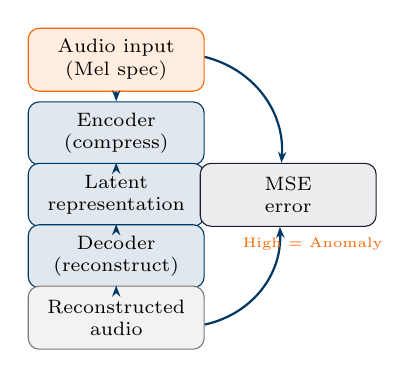
\begin{tikzpicture}[scale=0.78,font=\scriptsize]
        \node[obox,text width=2cm] (inp) at (0,2) {Audio input\\(Mel spec)};
        \node[pbox,text width=2cm] (enc) at (0,0.8) {Encoder\\(compress)};
        \node[pbox,text width=2cm] (lat) at (0,-0.2) {Latent\\representation};
        \node[pbox,text width=2cm] (dec) at (0,-1.2) {Decoder\\(reconstruct)};
        \node[gbox,text width=2cm] (out) at (0,-2.2) {Reconstructed\\audio};
        \node[dbox,text width=2cm] (mse) at (2.8,-0.2) {MSE\\ error};
        \draw[arr] (inp)--(enc); \draw[arr] (enc)--(lat);
        \draw[arr] (lat)--(dec); \draw[arr] (dec)--(out);
        \draw[arr] (inp) to[bend left=40] (mse);
        \draw[arr] (out) to[bend right=40] (mse);
        \node[font=\tiny,NXPOrange] at (3.2,-1.0) {High = Anomaly};
      \end{tikzpicture}
    \end{columns}
\end{frame}

%% ═══════════════════════════════════════════════════════════════════
\section{EEG / BCI}
%% ═══════════════════════════════════════════════════════════════════

\begin{frame}{EEG TCNet — Brain-Computer Interface (Unique Model)}
  \begin{columns}[T]
    \column{0.52\textwidth}
      \begin{block}{Model Information}
        \begin{itemize}\small
          \item Architecture: Temporal Convolutional Network (TCN)
          \item Input: EEG signal $(1 \times 1 \times 22 \times 1125)$\\\scriptsize(22 EEG channels, 4.5s at 250Hz)
          \item Output: 4-class motor imagery\\
            \scriptsize\textit{left hand / right hand / feet / tongue}
          \item Dataset: BCI Competition IV-2a
          \item Accuracy: \alert{77.35\%} (4-class)
          \item FLOPS: \alert{14 MOPS}, Params: \alert{4,096}
          \item 9 per-subject models trained
        \end{itemize}
      \end{block}
      \vspace{4pt}
      \begin{alertblock}{Only Zoo with EEG/BCI}
        TI and ADI model zoos have no EEG or BCI models. NXP targets \textbf{medical \& accessibility} applications.
      \end{alertblock}
    \column{0.44\textwidth}
      \begin{block}{TCN Architecture}
        \begin{itemize}\scriptsize
          \item Temporal convolutions with dilated receptive field
          \item Causal convolutions (no future context)
          \item Residual skip connections
          \item Compact: fits in 16KB — MCU-deployable
          \item From ETH Zurich IIS lab
        \end{itemize}
      \end{block}
      \vspace{4pt}
      \begin{block}{Limitations}
        \begin{itemize}\scriptsize
          \item NPU acceleration \textbf{not supported} on i.MX 8M Plus (LF6.1.36)
          \item Must use CPU inference
          \item Per-subject training required for high accuracy
          \item i.MX 8M Plus only
        \end{itemize}
      \end{block}
  \end{columns}
\end{frame}

%% ═══════════════════════════════════════════════════════════════════
\section{eIQ Toolkit}
%% ═══════════════════════════════════════════════════════════════════

\begin{frame}{eIQ Toolkit Ecosystem}
  \begin{columns}[T]
    \column{0.52\textwidth}
      \begin{block}{eIQ Toolkit Components}
        \begin{description}[\textbf{eIQ Portal}]\small
          \item[\textbf{TFLite Runtime}] ArmNN + XNNPACK delegates for i.MX NPU acceleration
          \item[\textbf{Ethos-U Delegate}] Hardware-accelerated inference on i.MX 93 Ethos-U65
          \item[\textbf{Vela Compiler}] Compiles TFLite $\to$ Ethos-U optimized binary (\texttt{nxp-imx/ethos-u-vela})
          \item[\textbf{eIQ Portal}] GUI tool for model deployment and profiling
          \item[\textbf{eIQ Examples}] Reference apps (\texttt{nxp-imx/eiq-examples})
        \end{description}
      \end{block}
    \column{0.44\textwidth}
      \begin{block}{Key Resources}
        \begin{itemize}\scriptsize
          \item \textbf{i.MX ML User Guide:}\\
            \texttt{nxp.com/docs/en/user-guide/}\\
            \texttt{IMX-MACHINE-LEARNING-UG.pdf}
          \item \textbf{eIQ Portal:} GUI model profiling, benchmark visualization
          \item \textbf{benchmark-model:} TFLite benchmark CLI (used for all model latency measurements)
          \item \textbf{BSP:} Yocto-based Linux BSP for i.MX 8M Plus and i.MX 93
        \end{itemize}
      \end{block}
      \vspace{4pt}
      \begin{alertblock}{Note}
        \scriptsize All model latency figures in the zoo are measured using \texttt{benchmark-model} — comparable across platforms.
      \end{alertblock}
  \end{columns}
\end{frame}

\begin{frame}{eIQ Deployment Workflow}
  \centering
  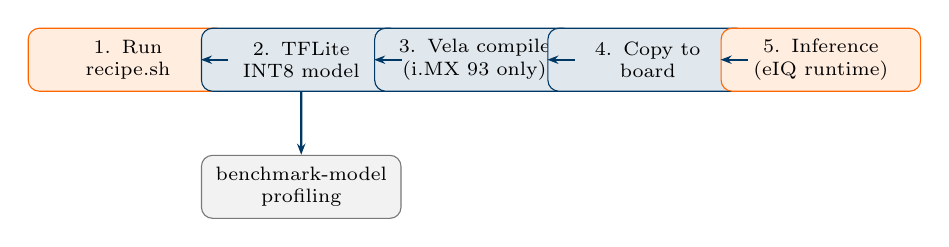
\begin{tikzpicture}[scale=0.85,font=\scriptsize,node distance=2.2cm]
    \node[obox,text width=2.3cm] (recipe) {1. Run\\recipe.sh};
    \node[pbox,text width=2.3cm,right of=recipe] (tfl) {2. TFLite\\INT8 model};
    \node[pbox,text width=2.3cm,right of=tfl] (vela) {3. Vela compile\\(i.MX 93 only)};
    \node[pbox,text width=2.3cm,right of=vela] (copy) {4. Copy to\\board};
    \node[obox,text width=2.3cm,right of=copy] (run) {5. Inference\\(eIQ runtime)};
    \draw[arr] (recipe)--(tfl);
    \draw[arr] (tfl)--(vela);
    \draw[arr] (vela)--(copy);
    \draw[arr] (copy)--(run);
    \node[gbox,text width=2.3cm,below=0.8cm of tfl] (bench) {benchmark-model\\profiling};
    \draw[arr] (tfl) -- (bench);
  \end{tikzpicture}
  \vspace{10pt}
  \begin{columns}[T]
    \column{0.48\textwidth}
      \begin{block}{Running Inference}
        \begin{lstlisting}[language=bash]
# On-board profiling
benchmark_model \
  --graph=model.tflite \
  --use_xnnpack=true

# With NPU delegate (i.MX 93)
benchmark_model \
  --graph=model_vela.tflite \
  --external_delegate_path=\
      ethosu_delegate.so
        \end{lstlisting}
      \end{block}
    \column{0.48\textwidth}
      \begin{block}{Example Python Inference}
        \begin{lstlisting}[language=python]
import tflite_runtime.interpreter \
    as tflite
interp = tflite.Interpreter(
    model_path="model.tflite")
interp.allocate_tensors()
inp = interp.get_input_details()
interp.set_tensor(inp[0]['index'],
    input_data)
interp.invoke()
        \end{lstlisting}
      \end{block}
  \end{columns}
\end{frame}

%% ═══════════════════════════════════════════════════════════════════
\section{MLOps Pipeline}
%% ═══════════════════════════════════════════════════════════════════

\begin{frame}{NXP eIQ MLOps Pipeline — Overview}
  \centering
  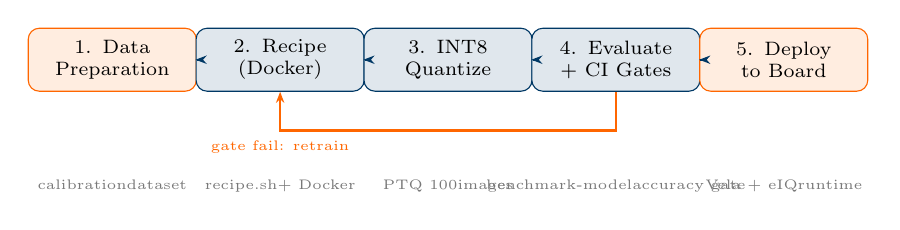
\begin{tikzpicture}[scale=0.82,font=\scriptsize]
    \node[obox,text width=1.9cm] (data)    at (0,0)    {1. Data\\Preparation};
    \node[pbox,text width=1.9cm] (recipe)  at (2.6,0)  {2. Recipe\\(Docker)};
    \node[pbox,text width=1.9cm] (quant)   at (5.2,0)  {3. INT8\\Quantize};
    \node[pbox,text width=1.9cm] (eval)    at (7.8,0)  {4. Evaluate\\+ CI Gates};
    \node[obox,text width=1.9cm] (deploy)  at (10.4,0) {5. Deploy\\to Board};
    \draw[arr] (data)--(recipe);
    \draw[arr] (recipe)--(quant);
    \draw[arr] (quant)--(eval);
    \draw[arr] (eval)--(deploy);
    %% Feedback
    \draw[oarr] (eval.south) -- ++(0,-0.6) -| node[below,midway,font=\tiny,NXPOrange]{gate fail: retrain} (recipe.south);
    %% Labels below
    \node[font=\tiny,NXPGray,below=1.0cm of data]   {calibration\\dataset};
    \node[font=\tiny,NXPGray,below=1.0cm of recipe]  {recipe.sh\\+ Docker};
    \node[font=\tiny,NXPGray,below=1.0cm of quant]   {PTQ 100\\images};
    \node[font=\tiny,NXPGray,below=1.0cm of eval]    {benchmark-model\\accuracy gate};
    \node[font=\tiny,NXPGray,below=1.0cm of deploy]  {Vela + eIQ\\runtime};
  \end{tikzpicture}
  \vspace{8pt}
  \begin{columns}[T]
    \column{0.48\textwidth}
      \begin{block}{MLOps Pillars}
        \begin{itemize}\scriptsize
          \item \textbf{Reproducibility}: Docker recipes pin all deps
          \item \textbf{Auditability}: \texttt{SBOM-1.5.spdx.json} for supply chain
          \item \textbf{Portability}: Same TFLite model, 5 platforms
          \item \textbf{CI integration}: GitHub Actions matrix per task $\times$ platform
        \end{itemize}
      \end{block}
    \column{0.48\textwidth}
      \begin{block}{Automation Scope}
        \begin{itemize}\scriptsize
          \item Lint + YAML validation
          \item Unit tests (preprocessing, evaluator)
          \item Per-task accuracy gate check
          \item Artifact packaging for deployment
        \end{itemize}
      \end{block}
  \end{columns}
\end{frame}

\begin{frame}[fragile]{Model Registry \& Version Management}
  \begin{columns}[T]
    \column{0.50\textwidth}
      \begin{block}{\texttt{model\_registry.yaml} Structure}
        \begin{lstlisting}[language=bash]
models:
  yolov8_m:
    version: "1.0.0"
    task: object_detection
    domain: vision
    format: tflite
    input_size: [320, 320]
    input_type: float32
    num_classes: 80
    dataset: coco
    weight_file: "yolov8m_int8.tflite"
    model_path: "tasks/vision/
      object-detection/yolov8"
    size_mb: 26.1
    flops_gops: 78.9
    supported_platforms:
      - platform: imx8mp
        board: 8MPLUSLPD4-EVK
        delegate: xnnpack
      - platform: imx93
        board: IMX93EVKBOARD
        delegate: ethos_u65
        vela_required: true
    metrics:
      mAP_reported: 50.2
    status: production
        \end{lstlisting}
      \end{block}
    \column{0.46\textwidth}
      \begin{block}{\texttt{ModelManager} Python API}
        \begin{lstlisting}[language=python]
manager = ModelManager(
    "config/pipeline_config.yaml")

# Look up model path
path = manager.get_model_path(
    "yolov8_m", platform="imx8mp")

# List by task + platform
models = manager.list_models(
    task="object_detection",
    platform="imx93")

# Check Vela requirement
meta = manager.get_metadata("yolov8_m")
if meta["vela_required"]:
    compile_vela(path)

# Get accuracy
acc = manager.get_accuracy("ds_cnn")
print(acc["accuracy_reported"])
        \end{lstlisting}
      \end{block}
  \end{columns}
\end{frame}

\begin{frame}{Evaluation \& CI/CD Accuracy Gates}
  \begin{columns}[T]
    \column{0.50\textwidth}
      \begin{block}{Accuracy Gates per Task}
        \centering\scriptsize
        \begin{tabular}{lll}
          \toprule
          \textbf{Task} & \textbf{Metric} & \textbf{Min Threshold} \\
          \midrule
          Classification  & Top-1 Acc & 65\% \\
          Object Detection& mAP       & 30\% \\
          Segmentation    & mIoU      & 60\% \\
          Keyword Spotting& Accuracy  & 85\% \\
          ASR             & WER       & $\leq$15\% \\
          Anomaly Det.    & AUC       & 0.50 \\
          EEG/BCI         & Accuracy  & 70\% \\
          Super Resolution& PSNR      & 28 dB \\
          \bottomrule
        \end{tabular}
      \end{block}
      \vspace{4pt}
      \begin{block}{Gate Failure Action}
        Gate fail $\Rightarrow$ re-run recipe with more calibration data or switch quantization mode (full INT8 vs.\ float I/O)
      \end{block}
    \column{0.46\textwidth}
      \begin{block}{GitHub Actions CI Matrix}
        \begin{lstlisting}[language=yaml]
strategy:
  matrix:
    include:
      - domain: vision
        task: object_detection
        model: yolov8_m
        platform: imx8mp
      - domain: vision
        task: classification
        model: mobilenetv2
        platform: imx93
      - domain: audio
        task: keyword_spotting
        model: ds_cnn
        platform: imx8mp
      - domain: misc
        task: eeg_bci
        model: eeg_tcnet
        platform: imx8mp
        \end{lstlisting}
      \end{block}
  \end{columns}
\end{frame}

\begin{frame}{\texttt{code-nxp/} Directory Structure}
  \begin{columns}[T]
    \column{0.50\textwidth}
      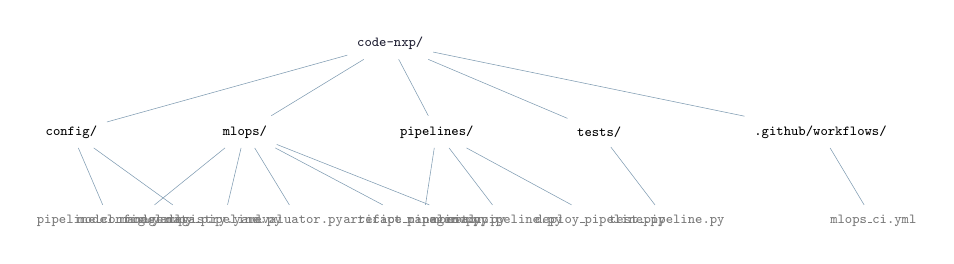
\begin{tikzpicture}[scale=0.75,font=\tiny,
          every node/.style={anchor=west},
          edge from parent/.style={draw=NXPBlue!50,very thin}]
        \node[NXPDark] {\texttt{code-nxp/}}
          child { node {\texttt{config/}}
            child { node[NXPGray] {\texttt{pipeline\_config.yaml}} }
            child { node[NXPGray] {\texttt{model\_registry.yaml}} } }
          child[missing] {}
          child { node {\texttt{mlops/}}
            child { node[NXPGray] {\texttt{model\_manager.py}} }
            child { node[NXPGray] {\texttt{data\_pipeline.py}} }
            child { node[NXPGray] {\texttt{evaluator.py}} }
            child { node[NXPGray] {\texttt{artifact\_manager.py}} }
            child { node[NXPGray] {\texttt{monitor.py}} } }
          child[missing] {}
          child { node {\texttt{pipelines/}}
            child { node[NXPGray] {\texttt{recipe\_pipeline.py}} }
            child { node[NXPGray] {\texttt{eval\_pipeline.py}} }
            child { node[NXPGray] {\texttt{deploy\_pipeline.py}} } }
          child[missing] {}
          child { node {\texttt{tests/}}
            child { node[NXPGray] {\texttt{test\_pipeline.py}} } }
          child[missing] {}
          child { node {\texttt{.github/workflows/}}
            child { node[NXPGray] {\texttt{mlops\_ci.yml}} } };
      \end{tikzpicture}
    \column{0.46\textwidth}
      \small
      \begin{tabular}{ll}
        \toprule
        \textbf{Module} & \textbf{Responsibility} \\
        \midrule
        \texttt{model\_manager} & Registry, path resolution, \\
                                & Vela flag lookup \\
        \texttt{data\_pipeline} & Multi-domain preprocessing \\
                                & (vision/audio/EEG) \\
        \texttt{evaluator}      & Accuracy gates, TFLite \\
                                & inference wrapper \\
        \texttt{artifact\_mgr}  & Bundle pack/verify \\
        \texttt{monitor}        & Latency, drift tracking \\
        \texttt{recipe\_pipeline} & Docker recipe orchestration \\
        \texttt{eval\_pipeline} & CI evaluation runner \\
        \texttt{deploy\_pipeline} & Vela + board deploy \\
        \bottomrule
      \end{tabular}
      \vspace{4pt}
      \begin{lstlisting}[language=bash]
# Run all models on imx8mp
python pipelines/eval_pipeline.py \
  --config config/pipeline_config.yaml \
  --platform imx8mp --all-models
      \end{lstlisting}
  \end{columns}
\end{frame}

%% ═══════════════════════════════════════════════════════════════════
\section{Comparison}
%% ═══════════════════════════════════════════════════════════════════

\begin{frame}{Three Model Zoos Compared}
  \centering\small
  \begin{tabular}{lccc}
    \toprule
    \textbf{Dimension} & \textbf{NXP eIQ} & \textbf{TI EdgeAI} & \textbf{ADI Model Zoo} \\
    \midrule
    Model count    & $\sim$35              & \alert{180+}    & $\sim$15 \\
    Domains        & Vision+Audio+Misc     & Vision only     & Vision+Audio+Sensor \\
    Format         & \alert{TFLite only}   & ONNX+TFLite+TVM & AI8X+TFLite+PyTorch \\
    Hardware       & MPU + MCU             & SoC/MPU         & MCU/DSP \\
    TOPS range     & 0.5--2.3              & 1--32           & $<$0.1 \\
    \midrule
    Unique tasks   & SR, Low-light,        & ADAS BEV,       & Motor fault, \\
                   & EEG/BCI, ASR          & 3D detection    & biosignal \\
    Deployment     & Docker recipe         & TIDL compiler   & ai8xize synthesis \\
    Storage        & Recipes (no weights)  & .link files     & Weights in repo \\
    NPU type       & Ethos-U65 / NXP       & MMA + C7x DSP   & CNN accelerator \\
    \midrule
    Best for       & \textbf{Broad tasks,} & \textbf{ADAS,}  & \textbf{Sensor,} \\
                   & \textbf{Linux MPU}    & \textbf{vision} & \textbf{ultra-low power} \\
    \bottomrule
  \end{tabular}
\end{frame}

\begin{frame}{TOPS Comparison Across All Three Zoos}
  \centering
  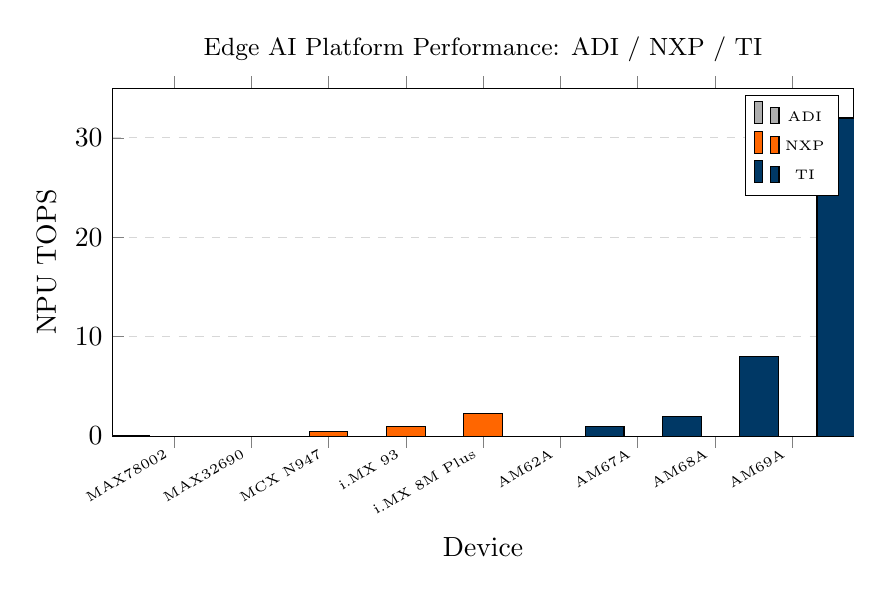
\begin{tikzpicture}
    \begin{axis}[
      width=11cm, height=6cm,
      ybar, bar width=14pt,
      xlabel={Device},
      ylabel={NPU TOPS},
      symbolic x coords={MAX78002,MAX32690,MCX N947,i.MX 93,i.MX 8M Plus,AM62A,AM67A,AM68A,AM69A},
      xtick=data,
      x tick label style={rotate=30,anchor=east,font=\tiny},
      ymin=0, ymax=35,
      ymajorgrids, grid style={dashed,NXPGray!30},
      title={\small Edge AI Platform Performance: ADI / NXP / TI},
      legend style={at={(0.98,0.98)},anchor=north east,font=\tiny},
    ]
    \addplot[fill=NXPGray!60] coordinates {
      (MAX78002,0.04)(MAX32690,0.001)(MCX N947,0)(i.MX 93,0)(i.MX 8M Plus,0)(AM62A,0)(AM67A,0)(AM68A,0)(AM69A,0)};
    \addplot[fill=NXPOrange] coordinates {
      (MAX78002,0)(MAX32690,0)(MCX N947,0.5)(i.MX 93,1.0)(i.MX 8M Plus,2.3)(AM62A,0)(AM67A,0)(AM68A,0)(AM69A,0)};
    \addplot[fill=NXPBlue] coordinates {
      (MAX78002,0)(MAX32690,0)(MCX N947,0)(i.MX 93,0)(i.MX 8M Plus,0)(AM62A,1)(AM67A,2)(AM68A,8)(AM69A,32)};
    \legend{ADI,NXP,TI}
    \end{axis}
  \end{tikzpicture}
\end{frame}

%% ═══════════════════════════════════════════════════════════════════
\section{Summary}
%% ═══════════════════════════════════════════════════════════════════

\begin{frame}{Key Takeaways}
  \begin{columns}[T]
    \column{0.48\textwidth}
      \begin{block}{Strengths of NXP eIQ Model Zoo}
        \begin{itemize}
          \item \alert{Broadest task coverage} of the three zoos (9 vision + audio + EEG)
          \item \alert{TFLite standard} — no proprietary format, portable
          \item \alert{Recipe system} ensures reproducible FP32$\to$INT8 pipeline
          \item \alert{Ethos-U65 NPU} support via Vela on i.MX 93
          \item \alert{SBOM} included for supply chain transparency
          \item Only zoo with \textbf{EEG/BCI}, \textbf{ASR}, \textbf{super resolution}, and \textbf{low-light enhancement}
        \end{itemize}
      \end{block}
    \column{0.48\textwidth}
      \begin{block}{Best Fit Use Cases}
        \begin{itemize}
          \item Smart home / security cameras (i.MX 8M Plus)
          \item Industrial inspection (i.MX 93 + Ethos-U)
          \item ADAS driver monitoring (WHENet, face landmarks)
          \item Medical / accessibility (EEG TCNet)
          \item IoT edge nodes (MCX N947)
          \item Embedded ASR endpoints (Wav2Letter on i.MX 93)
        \end{itemize}
      \end{block}
  \end{columns}
  \vspace{6pt}
  \begin{alertblock}{Compared to TI and ADI}
    NXP eIQ sits between TI (high TOPS, ADAS-focused, 180+ models) and ADI (ultra-low power MCU, sensor-domain). NXP offers the widest task variety with a hardware-neutral TFLite format.
  \end{alertblock}
\end{frame}

\begin{frame}{Getting Started \& Next Steps}
  \begin{columns}[T]
    \column{0.48\textwidth}
      \begin{block}{Quick Start (5 minutes)}
        \begin{enumerate}\small
          \item Clone the repo:
            \\\texttt{git clone https://github.com/NXP/eiq-model-zoo}
          \item Build Docker image:
            \\\texttt{docker build -t nxp-model-zoo .}
          \item Run a recipe:
            \\\texttt{cd tasks/vision/object-detection/yolov8}
            \\\texttt{docker run --rm -v "\$PWD:/workspace" nxp-model-zoo recipe.sh}
          \item Copy \texttt{.tflite} to board and benchmark
        \end{enumerate}
      \end{block}
    \column{0.48\textwidth}
      \begin{block}{Next Steps}
        \begin{itemize}\small
          \item \textbf{Profile with eIQ Portal} — visualize layer latencies
          \item \textbf{Fine-tune} — find original model source in recipe, retrain on your data
          \item \textbf{Vela compile} — enable Ethos-U65 NPU on i.MX 93
          \item \textbf{Explore EEG TCNet} — first EEG model in production embedded AI
          \item \textbf{Multi-model pipeline} — chain FaceDet $\to$ Facenet512 for face verification
          \item \textbf{Run code-nxp/ MLOps pipeline} — automate recipe + evaluation
        \end{itemize}
      \end{block}
  \end{columns}
  \vspace{8pt}
  \centering
  \textbf{Repository:} \texttt{https://github.com/NXP/eiq-model-zoo}
  \quad \textbf{eIQ Portal:} \texttt{nxp.com/eiq}
\end{frame}

\end{document}
